\chapter{Análisis de textos médicos}

En este capítulo discutiremos cómo hemos llevado a cabo la evaluación de las herramientas disponibles en el estado del arte para la extracción de información en texto no estructurado de carácter médico.

Para ello se ha creado una web app disponible de forma muy accesible para que sea fácil ver el poder combinado de todas estas herramientas. Dicha herramienta se denomina \href{https://share.streamlit.io/jesi-rgb/medical-text-analysis/src/streamlit_gen_test.py}{MEDGEN}.



\section{Despliegue de MEDGEN}

Para hacer accesible todo el trabajo que se ha acometido, se ha elaborado una aplicación que permite hacer uso de todas las técnicas y herramientas discutidas a lo largo del documento. 

El framework utilizado ha sido \href{https://streamlit.io}{Streamlit}. Streamlit es un framework para Python diseñado para el prototipado ágil de aplicaciones web. Los creadores idearon esta herramienta para disminuir el esfuerzo que hay que acometer a la hora de desplegar una aplicación basada en inteligencia artificial, es decir, una aplicación que consta de sistemas de inferencia o similares, sistemas que no se encuentran en aplicaciones web usuales. 

De esta forma, es muy accesible y sencillo diseñar una aplicación en Python, donde se puede integrar cualquier sistema de IA en desarrollo y habilitar un espacio para que personas ajenas al desarrollo experimenten de primera mano cómo funciona, ofreciendo la oportunidad de crear casos de uso reales.

La aplicación permite generar comentarios utilizando el modelo generativo, y permite analizar dichos comentarios, así como importar desde distintas fuentes. La aplicación efectúa un pequeño análisis del texto y utiliza el tagger que el usuario seleccione.

\section{Evaluación de las herramientas}

Como vemos en las Figuras \ref{fig:app-demo} y \ref{fig:analysis-comment}, podemos efectuar nuestro análisis de diferentes formas. La aplicación nos permite utilizar los NER Taggers indicados en la Sección \ref{sec:nertagger}: Med7, BC5CDR y BIONLP13CG.

Podemos, en caso de no disponer de un conjunto de datos, generar comentarios usando nuestro modelo generativo. Una vez generados, podemos analizarlos con el NER Tagger que deseemos. Aquí, el desarrollador estaría programando el suyo propio y podría integrarlo al sistema fácilmente para testearlo de forma apropiada. 

El análisis nos ofrece una versión etiquetada del texto original, así como unas estadísticas del comentario en concreto. Además de ello, podemos importar nuestros propios comentarios desde un archivo o copiarlos y pegarlos en el campo de texto, con tal de maximizar la comodidad de uso de la aplicación.

En función del texto de entrada y el Tagger seleccionado obtendremos mejores o peores resultados. El generador de comentarios está entrenado para generar comentarios de carácter quirúrgico o posoperatorios. Para ello, el BIONLP13CG es una buena elección, pero el Med7 rara vez será capaz de ofrecer resultados, ya que está especializado en recetas médicas.

La ventaja de esto es el gran abanico de posibilidades que tenemos de forma muy accesible, siendo posible analizar casi cualquier tipo de texto médico que sea de interés. De no disponer de un Tagger apropiado, siempre podemos incluirlo en la aplicación, como mencionábamos en la Sección \ref{sec:nertagger}.

\begin{figure}[h]
	\centering
	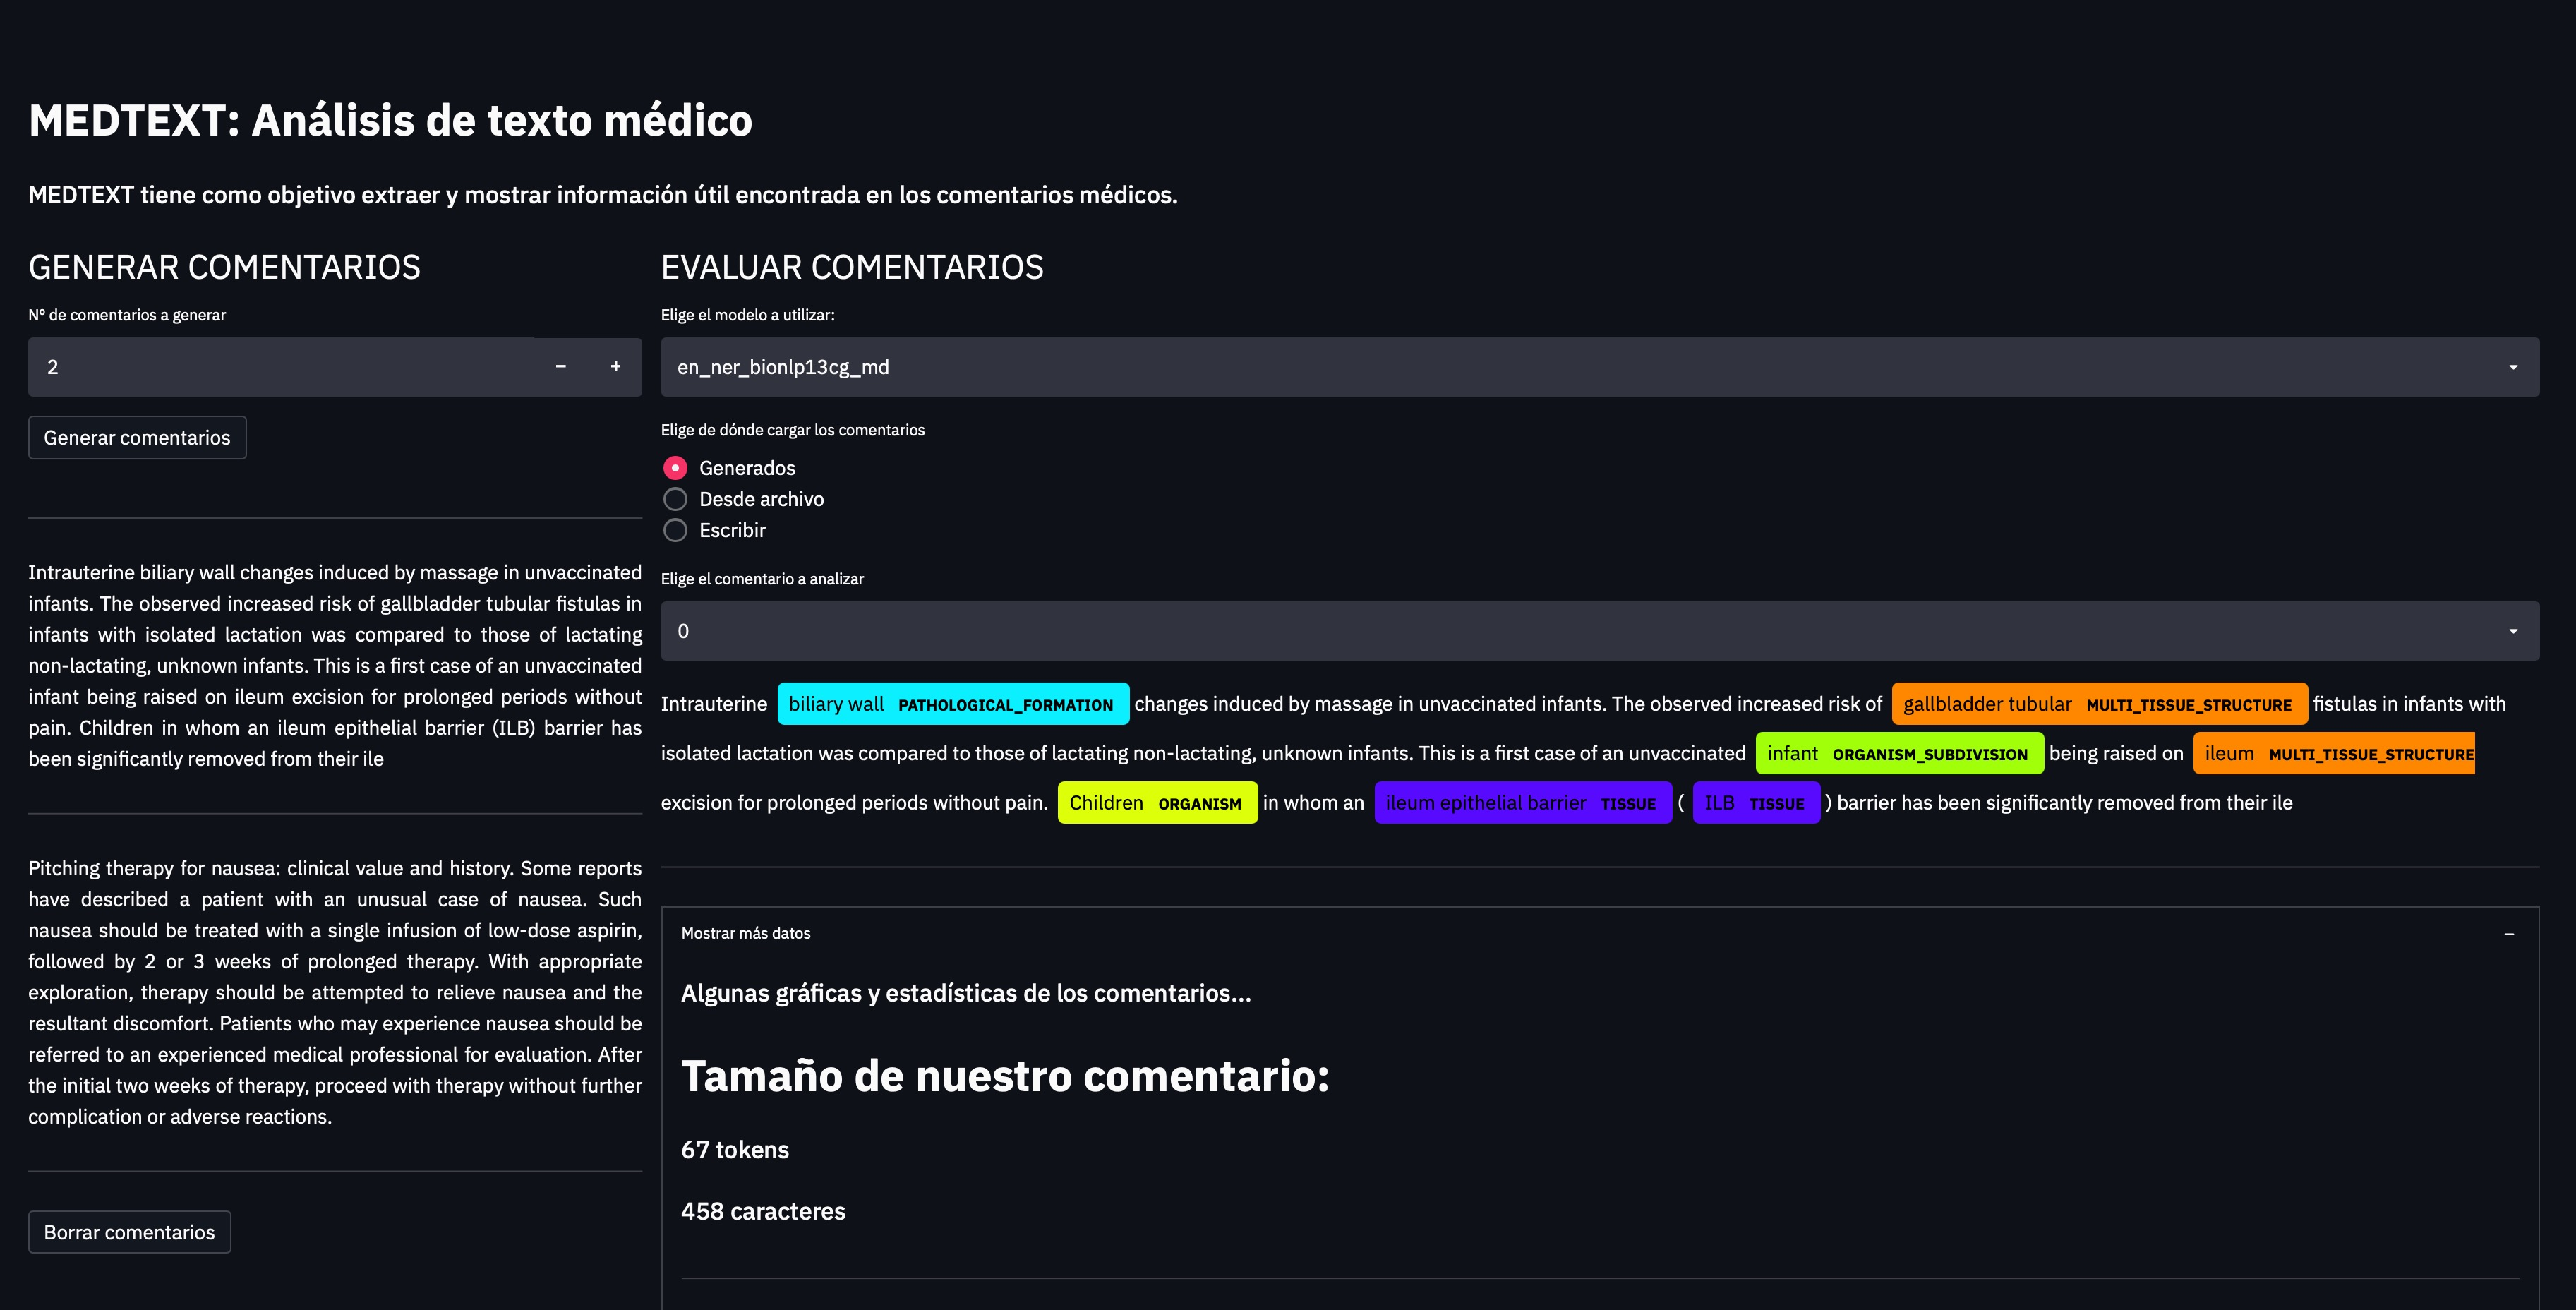
\includegraphics[width=.9\textwidth]{media/app_demo.jpeg}
	\caption{Captura de pantalla de la aplicación elaborada. A la izquierda podemos generar comentarios y a la derecha, analizarlos.}
	\label{fig:app-demo}
\end{figure}


\begin{figure}[h]
	\centering
	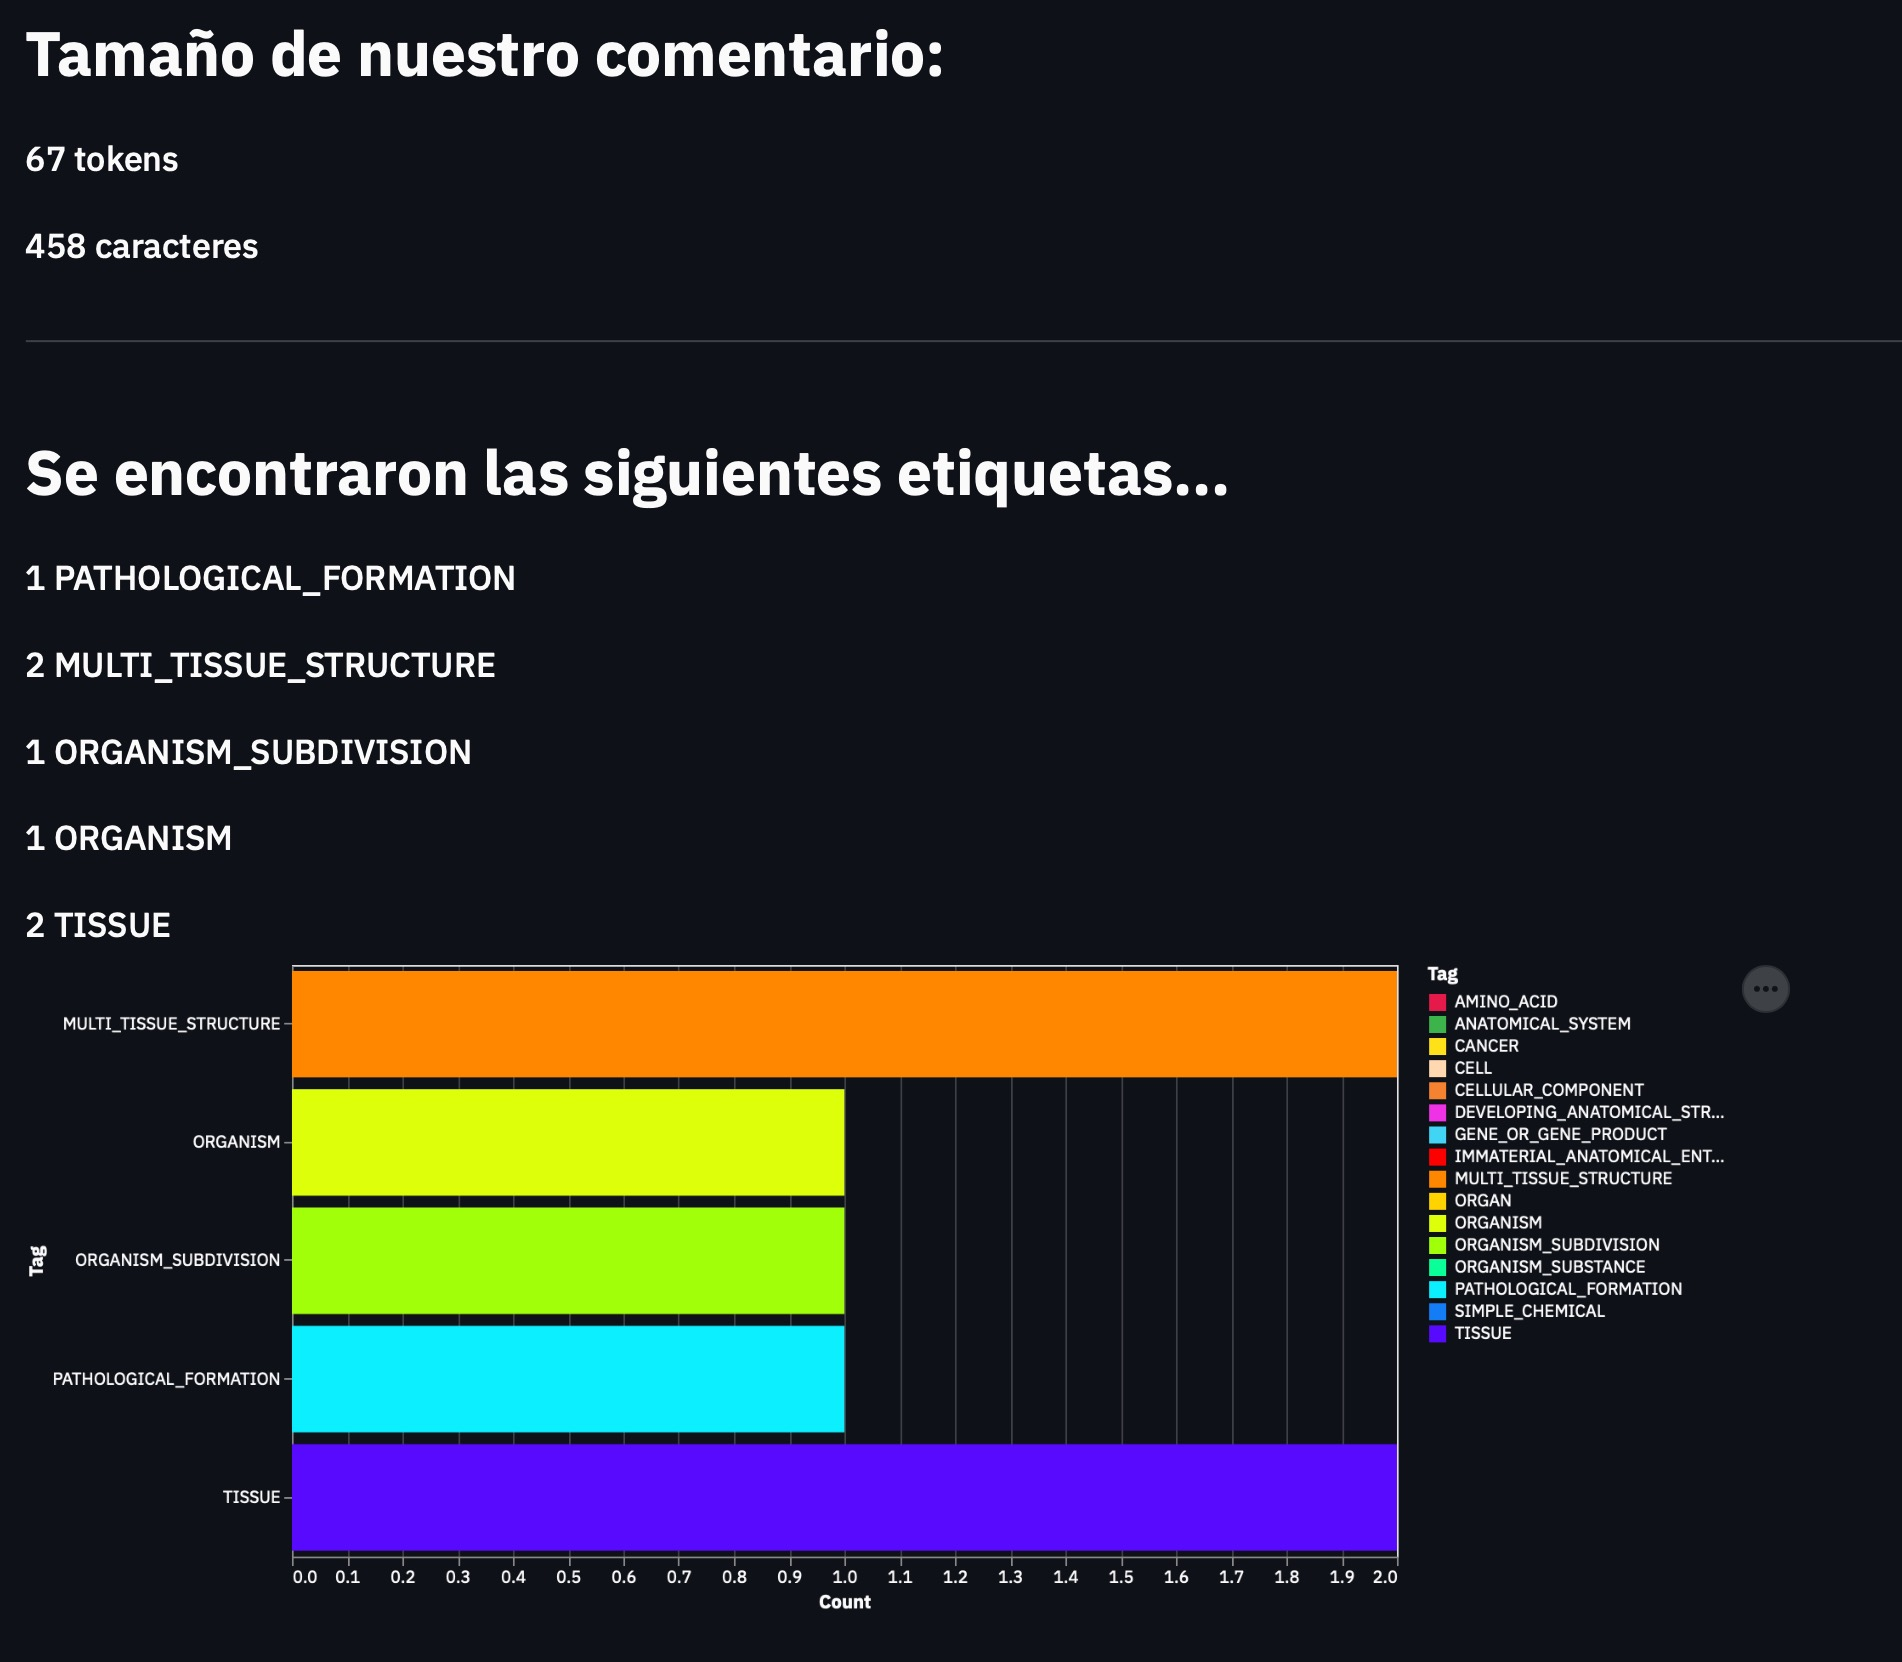
\includegraphics[width=.62\textwidth]{media/analysis_comment.jpeg}
	\caption{Captura de pantalla del análisis que ofrece la aplicación acerca de un determinado comentario.}
	\label{fig:analysis-comment}
\end{figure}



\section{Instalación y modo de uso}
La aplicación puede compilarse desde el código fuente siguiendo el \href{https://github.com/jesi-rgb/medical-text-analysis}{enlace al repositorio}, descargándolo y ejecutando los siguientes comandos:

\jesitt{git clone https://github.com/jesi-rgb/medical-text-analysis}

Activamos el entorno que más nos guste, ya sea de python o conda.

\jesitt{cd medical-text-analysis}

\jesitt{pip install -r requirements.txt}

Una vez finalizado, 

\jesitt{streamlit run src/streamlit\_gen\_test.py}

se nos abrirá una ventana en el navegador y la aplicación estará lista para funcionar.

La primera ejecución tarda un poco más, ya que ha de descargar el modelo de Internet y cargarlo en memoria. Tras eso, los modelos se guardan en caché y la ejecución es mucho más rápida.
